\chapter{Results and Discussion}

\section{Summary of Test Results}

The tested results yielded expected results - Ireland primarily blocked pirated and illegal content, while Iraq blocked a wider range of content.

[expanded stuff will go here]

\subsection{Website Accessibility Results}

The results below are an average of the number of websites blocked each day over the testing period of 15 days.

\begin{table}[H]
\centering
\caption{Summary of Blocked vs. Unblocked Websites by Country}
\begin{tabular}{lcc}
\toprule
\textbf{Country} & \textbf{Unblocked} & \textbf{Blocked} \\
\midrule
Ireland & X & Y \\
Iraq    & A & B \\
\bottomrule
\end{tabular}
\label{tab:blocked_summary}
\end{table}

The table below shows the frequency of block methods found in Iraq.

\begin{table}[H]
\centering
\caption{Distribution of Blocking Methods Detected in Iraq}
\begin{tabular}{lc}
\toprule
\textbf{Blocking Method} & \textbf{Frequency} \\
\midrule
TCP/IP          & N1 \\
DNS & N2 \\
HTTP & N3 \\
\bottomrule
\end{tabular}
\label{tab:iraq_blocking_methods}
\end{table}

The table below shows the frequency of block methods found in Ireland.

\begin{table}[H]
\centering
\caption{Distribution of Blocking Methods Detected in Ireland}
\begin{tabular}{lc}
\toprule
\textbf{Blocking Method} & \textbf{Frequency} \\
\midrule
TCP/IP          & N1 \\
DNS & N2 \\
HTTP & N3 \\
Unidentified & N3 \\
\bottomrule
\end{tabular}
\label{tab:ireland_blocking_methods}
\end{table}

The table below shows the number of websites blocked in each category in both countries.

\begin{table}[H]
\centering
\caption{Blocked Websites by Category and Country}
\begin{tabular}{lcc}
\toprule
\textbf{Category} & \textbf{Ireland} & \textbf{Iraq} \\
\midrule
Uncategorized                       & -- & -- \\
Piracy / Streaming / File Sharing   & -- & -- \\
News / Media                        & -- & -- \\
Adult Content                       & -- & -- \\
Creative / Educational / Misc       & -- & -- \\
General / National Services         & -- & -- \\
Streaming / Social Media            & -- & -- \\
Religious                           & -- & -- \\
VoIP / Communication                & -- & -- \\
Gambling                            & -- & -- \\
Email/Privacy Tools                 & -- & -- \\
Adult / Alcohol                     & -- & -- \\
LGBTQ+                              & -- & -- \\
AI / Technology                     & -- & -- \\
\bottomrule
\end{tabular}
\label{tab:category_block}
\end{table}

\subsection{Circumvention Test Results}



\subsection{Instant Messaging Test Results}

The results of the Instant Messaging tests were very similar in Ireland and Iraq. Both tests showed signs of no interference of blocking of Facebook Messenger, Telegram, Whatsapp, or Signal. However, looking outside of the tested ASNs reveals a significant difference between the two countries. The tested data in Ireand is consistent with public OONI data, and shows no blocking of instant messaging platforms. The Iraq data is also consistent with tests run on the same ASN, but in Iraq there are other ASNs that show signs of blocking.

\subsubsection{Ireland}

In the past 30-day period, there were only 3 anomalies found that shows any kind of instant messaging blocking:

\textbf{March 24, 2025} - Packethub S.A. (AS136787) - Facebook Messenger Test
%https://explorer.ooni.org/m/20250324111124.418686_IE_facebookmessenger_fbdc8895400acaba

\textbf{March 24, 2025} - HEAnetCLG (AS1213) - Signal Test
%https://explorer.ooni.org/m/20250324164458.153631_IE_signal_667f7ad13e55043a

Outside of these anomalies, there was no evidence of instant messaging blocking.

\subsubsection{Iraq}

Iraq had significant evidence of instant messaging platforms being blocked in certain ASNs. The table below shows each ASN, and the percentage of tests where there was an anomaly found.

\begin{table}[H]
\centering
\caption{ASN's with Evidence of Instant Message Platform Blocking}
\begin{tabular}{lcccc}
\toprule
\textbf{ASN} & \textbf{Facebook} & \textbf{Telegram} & \textbf{WhatsApp} & \textbf{Signal} \\
\midrule
AS203214  & 27\%  & 7.8\% & 25\%  & 44\% \\
AS205254  & 26\%  & 3.8\% & 7.6\% & 7.6\% \\
AS199739  & 1\%   & 0.5\% & 0.2\% & 0.8\% \\
AS13335   & 47\%  & 0\%   & 0\%   & 0\% \\
AS50710   & 33\%  & 0\%   & 0\%   & 0\% \\
AS206206  & 60\%  & 0\%   & 0\%   & 0\% \\
AS212330  & 100\% & 0\%   & 0\%   & 0\% \\
AS210022  & 0\%   & 0\%   & 0\%   & 82\% \\
AS51020   & 0\%   & 0\%   & 0\%   & 32\% \\
AS202651  & 0\%   & 0\%   & 0\%   & 23\% \\
AS59588   & 0\%   & 0\%   & 1.9\% & 1.9\% \\
AS209193  & 0\%   & 0\%   & 0.7\% & 0\% \\
\bottomrule
\end{tabular}
\label{tab:category_block}
\end{table}

Instant Messaging platforms are essentially widely available in Iraq, but there are some areas where blocking does occur.

\subsection{Middlebox Test Results}

The results of the Middlebox Test were the same for both countries. Both the HTTP Header Field Manipulation and HTTP Invalid Request Line tests resulted in no Middleboxes being detected in either country. However, while there was no evidence of Middleboxes being found using the providers tested, it is possible that other providers in both countries have Middleboxes present in the network.

Using publicly available OONI data for Ireland and Iraq, it was found that there were cases of Middleboxes being detected in both countries over the past 30 days (March 6, 2025 - April 6, 2025). 

\subsubsection{Ireland}

There is very little evidence of Middleboxes being present in Ireland. Over the past 30-day period, there are only two anomalies present. Both of these anomalies are from the HTTP Invalid Request Line test. 

\textbf{March 25, 2025} - Meteor Mobile Communications Ireland (AS15751)
%https://explorer.ooni.org/m/20250325122211.663367_IE_httpinvalidrequestline_c713442d98eebb5c

\textbf{April 1, 2025} - Vodafone Ireland Limited (AS15502)
%https://explorer.ooni.org/m/20250401215651.365763_IE_httpinvalidrequestline_51f20fe7e9d31698

These results are likely outliers, as there are no other Middlebox tests for Meteor Mobile Communications Ireland in this time span and no other anomalies for Vodafone Ireland Limited.

\subsubsection{Iraq}

There is considerably more evidence of Middleboxes being present in Iraq. Over the past 30 day period, there were 125 anomalies in the HTTP Invalid request line Test and 19 anomalies in the HTTP Header Field Manipulation Test.

The table below lists the ASNs that were suspected to have Middleboxes present using the HTTP Invalid Request Line test. It then shows the number of anomalies, the total measurement count, and what percentage of the total count were anomalies. Note that any ASN that had less than 0.5\% anomalies was ignored.

\begin{table}[H]
\centering
\caption{ASN's with Evidence of Middleboxes (HTTP Invalid Request Line Test)}
\begin{tabular}{lccc}
\toprule
\textbf{ASN} & \textbf{Anomaly} & \textbf{Total Measurement Count} & \textbf{Percentage} \\
\midrule
AS13335   & 8 & 10 & 80\% \\
AS59588   & 13 & 53 & 24.5\% \\
AS48492   & 2 & 4 & 50\% \\
AS50710   & 1 & 1 & 100\% \\
AS198589  & 68 & 70 & 97\% \\
AS203214  & 32 & 158 & 20.25\% \\
\bottomrule
\end{tabular}
\label{tab:category_block}
\end{table}

\begin{figure}[H]
    \centering
    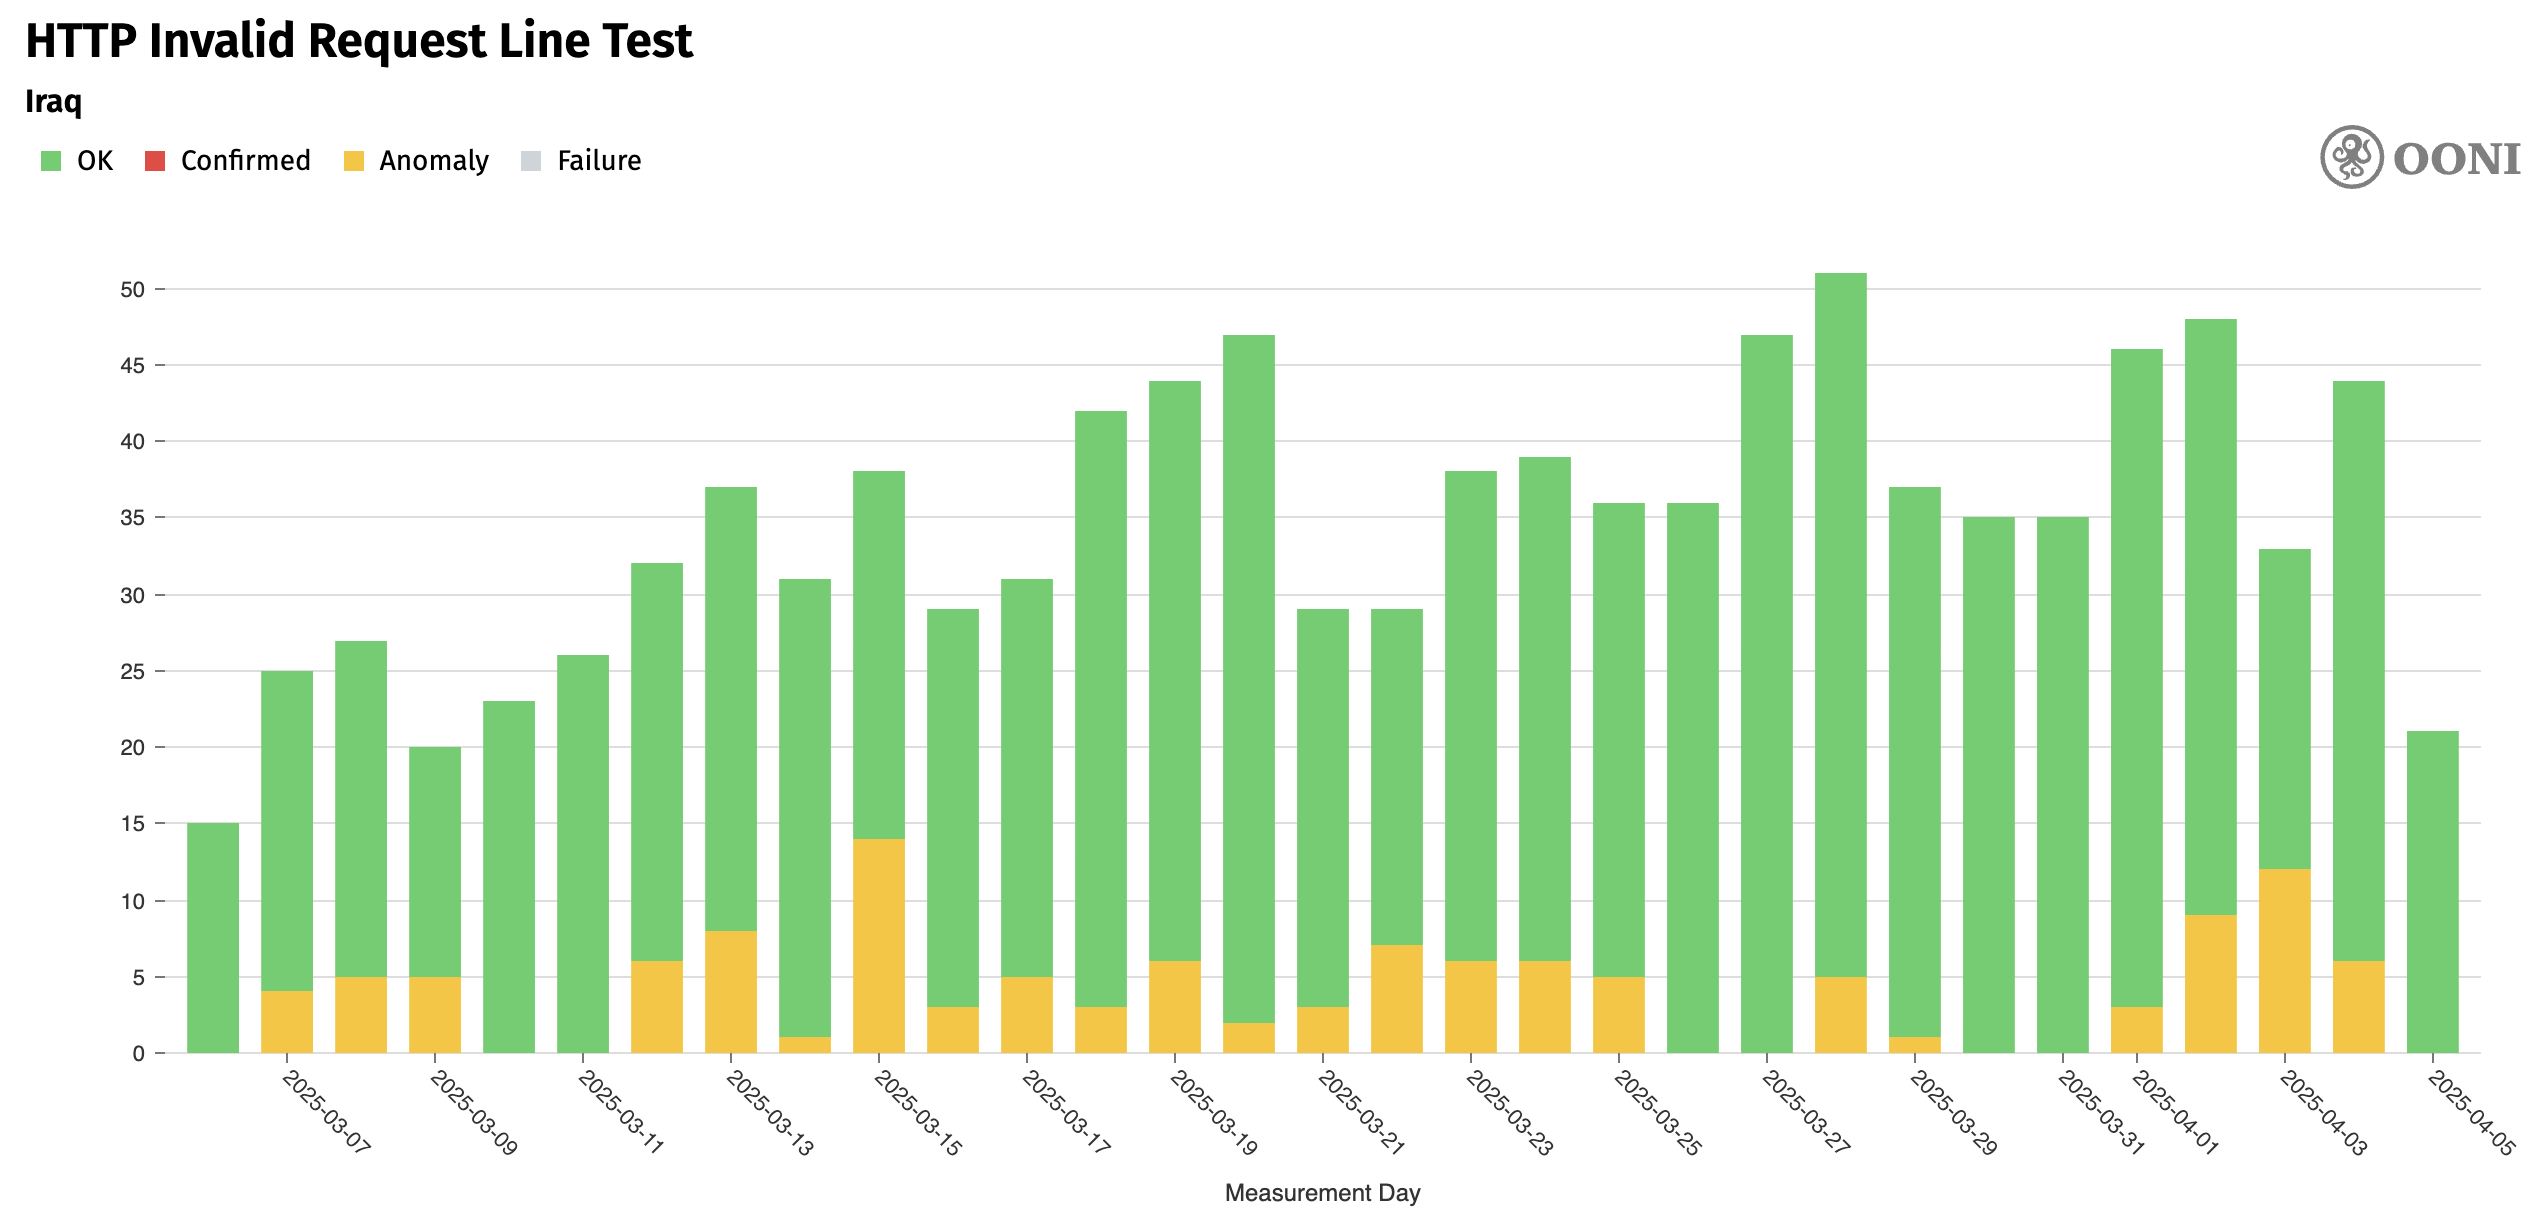
\includegraphics[width=\textwidth]{Griff/TCD SCSS CAPSTONE/Results/IraqMiddleboxHTTPInvalidTest.png}
    \caption{Iraq Middlebox HTTP Invalid Request Line Test: March 6, 2025 -- April 6, 2025}
    \label{fig:iraq-middlebox-invalid-request}
\end{figure}

The table below lists the ASNs that were suspected to have Middleboxes present using the HTTP Header Field Manipulation test. It then shows the number of anomalies, the total measurement count, and what percentage of the total count were anomalies. Note that any ASN that had less than 0.5\% anomalies was ignored.

\begin{table}[H]
\centering
\caption{ASN's with Evidence of Middleboxes (HTTP Header Field Manipulation Test)}
\begin{tabular}{lccc}
\toprule
\textbf{ASN} & \textbf{Anomaly} & \textbf{Total Measurement Count} & \textbf{Percentage} \\
\midrule
AS13335   & 8 & 10 & 80\% \\
AS48492   & 2 & 4 & 50\% \\
AS50710   & 1 & 1 & 100\% \\
\bottomrule
\end{tabular}
\label{tab:category_block}
\end{table}

\begin{figure}[H]
    \centering
    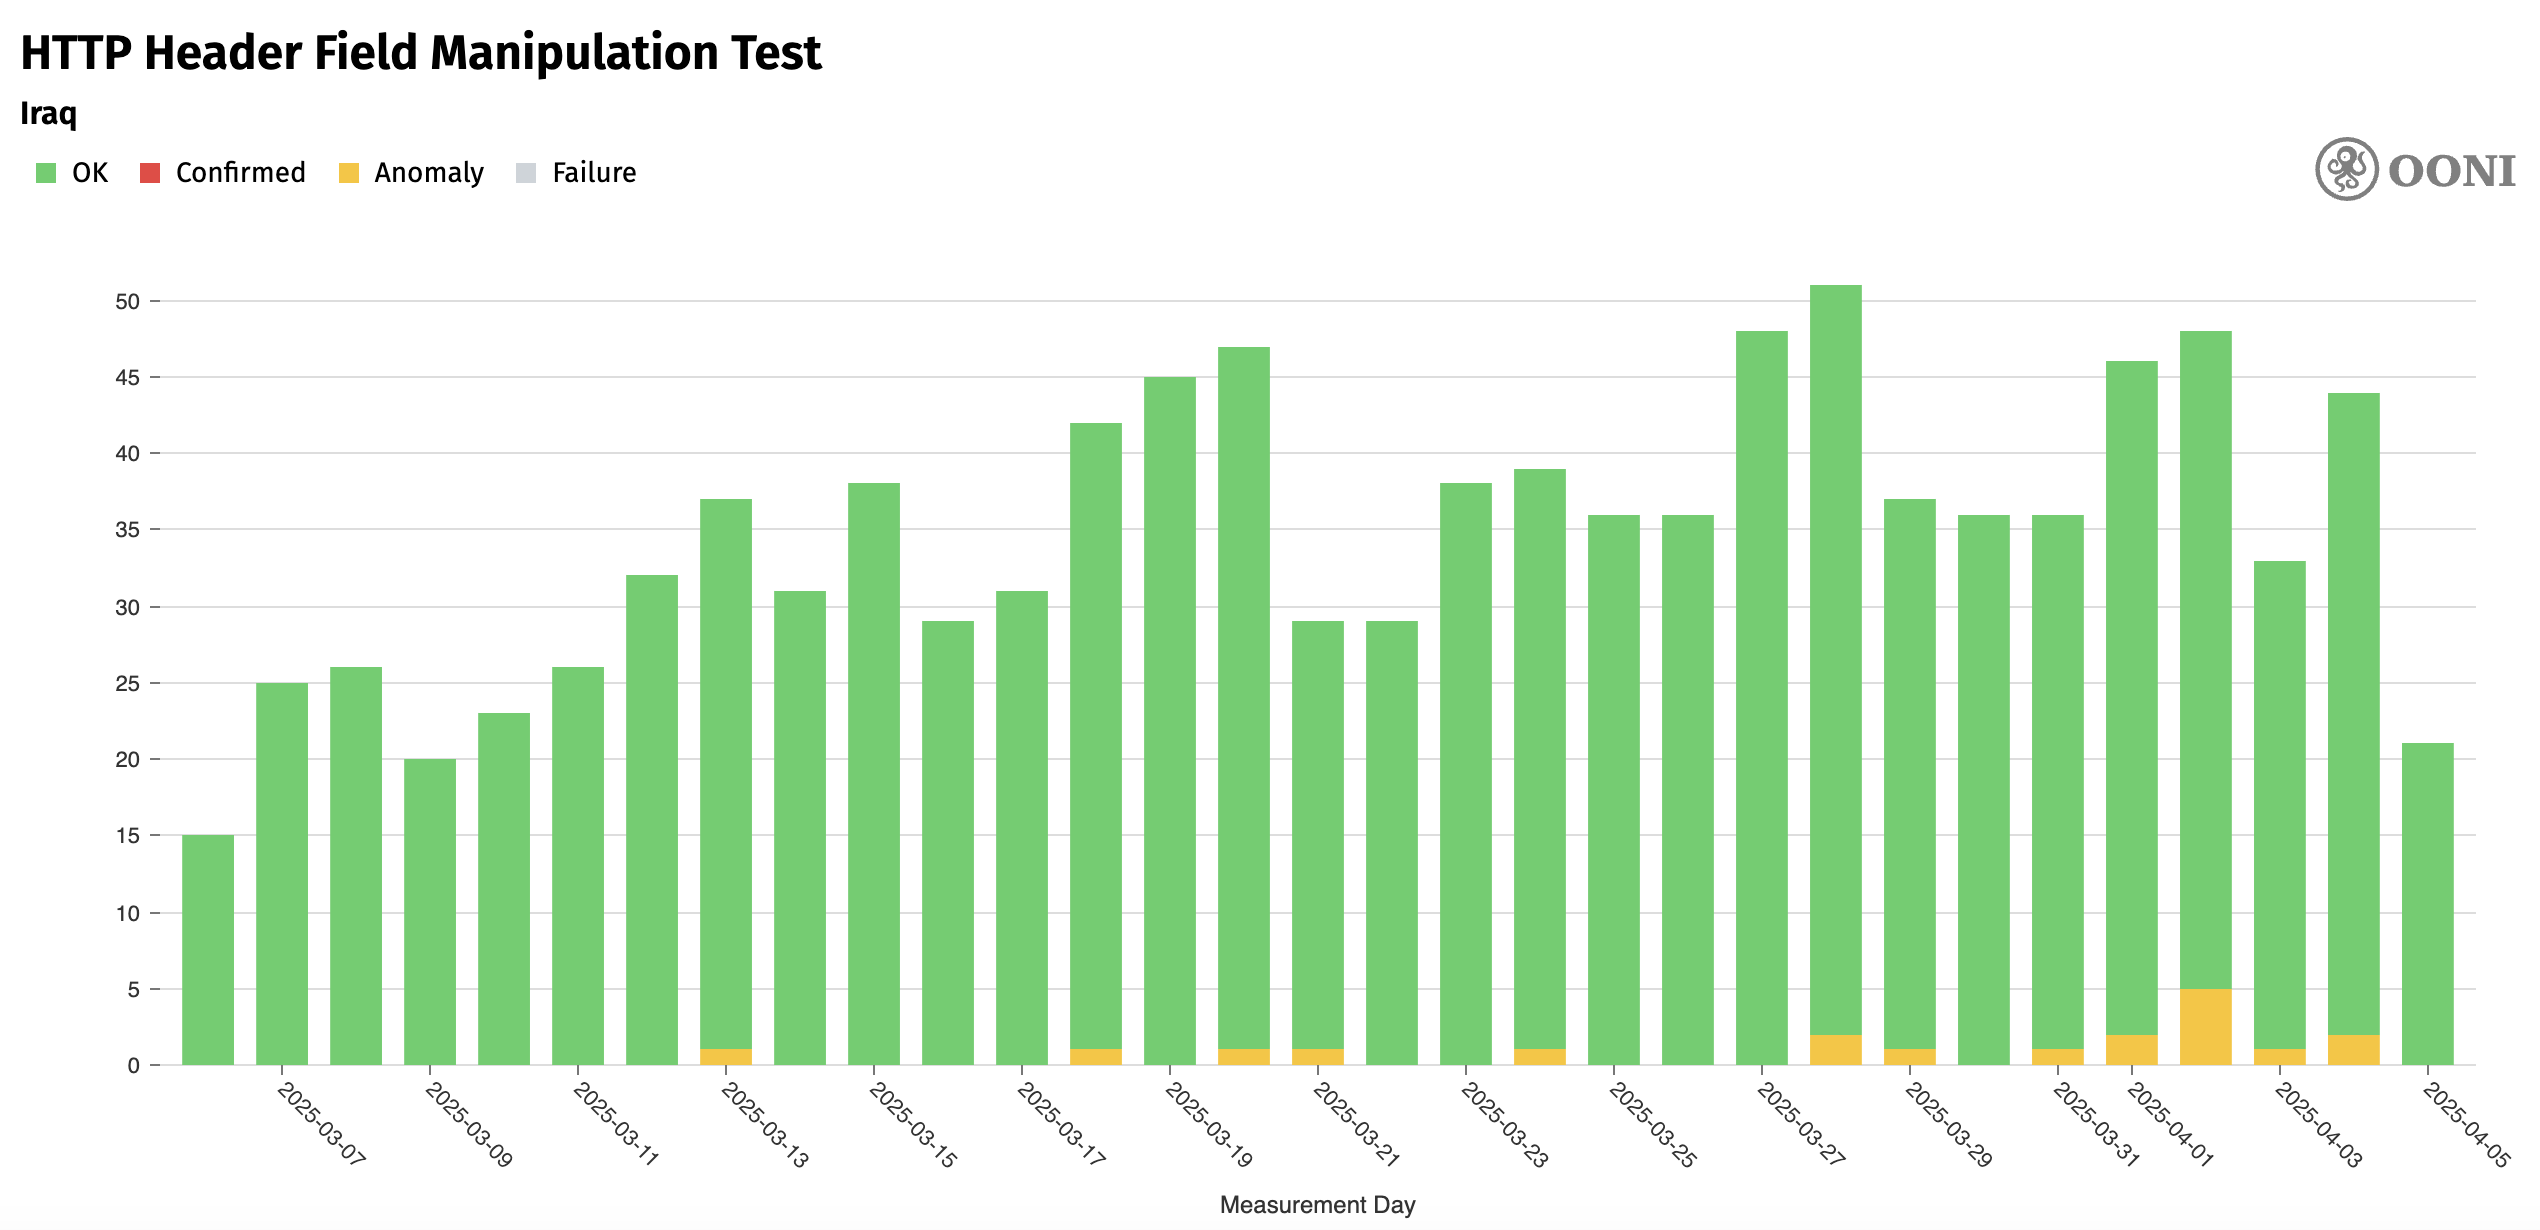
\includegraphics[width=\textwidth]{Griff/TCD SCSS CAPSTONE/Results/IraqMiddleboxHTTPManipulation.png}
    \caption{Iraq Middlebox HTTP Header Field Manipulation Test: March 6, 2025 -- April 6, 2025}
    \label{fig:iraq-middlebox-HTTP-manipulation}
\end{figure}

\textit{Note: All CSV files gathered from the public OONI database can be found on the public GitHub for this work; see Appendix A1.2.}


\section{Comparative Analysis: Ireland v. Iraq}



\subsection{Observed Patterns and Anomalies}



